\section{Permissões do Painel Administrativo}\label{RS0005:access}

\subsection{Introdução}

\subsubsection{Usuários}

\begin{figure}[!ht]
    \centering
    
\includegraphics[width=.8\textwidth]{usuarios}
\end{figure}

O Painel Administrativo do Portal Institucional possui um cadastro de usuários onde é possível acrescentar, atualizar ou remover usuários com acesso ao próprio painel.

\begin{figure}[!ht]
    \centering
    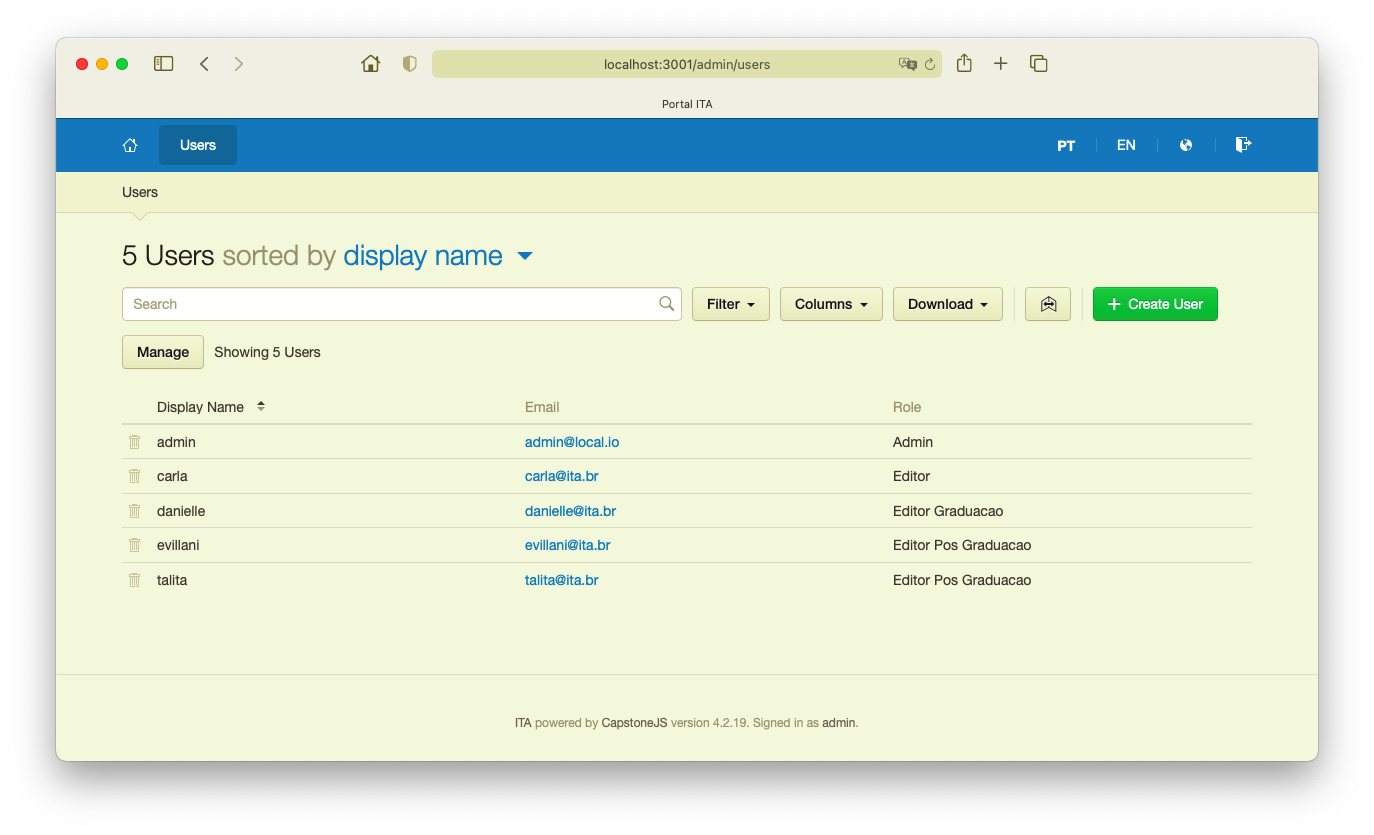
\includegraphics[width=.8\textwidth]{cadastro}
    \caption{Lista de usuários cadastrados}\label{RS0005:fig:cadastro}
\end{figure}

\begin{figure}[!ht]
    \centering
    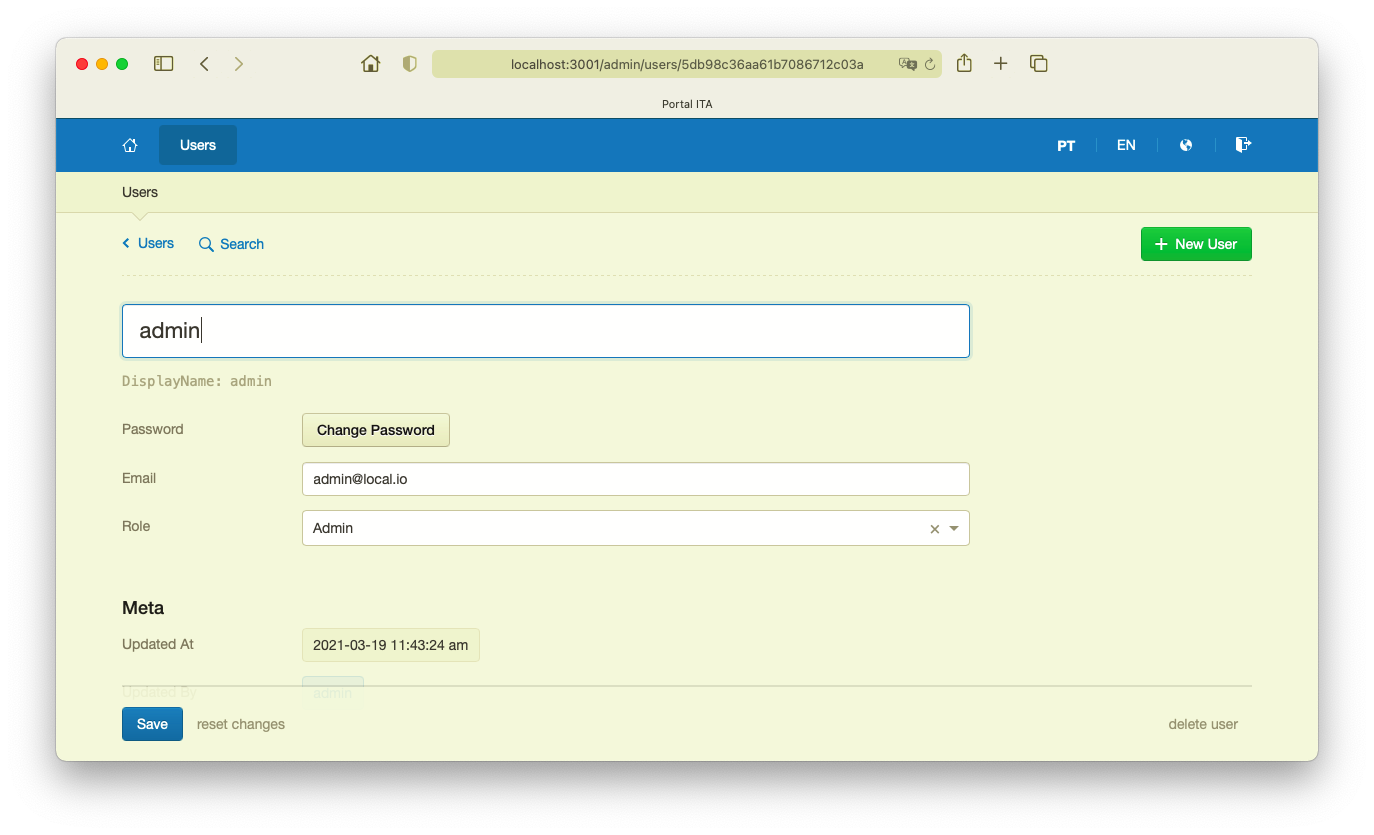
\includegraphics[width=.8\textwidth]{cadastro-usuario}
    \caption{Tela do cadastro de usuários}\label{RS0005:fig:cadastro-usuario}
\end{figure}

Além do cadastro de usuários no Painel Administrativo, também existe o serviço \gls{LDAP}\cite{howes2003understanding}, onde é feita a associação do usuário com as permissões deste no Painel. Para cadastrar um usuário no \gls{LDAP} é possível usar um arquivo \gls{LDIF}\cite{good2000rfc2849}, porém a forma de fazê-lo não importa, desde que algumas informações entre as partes sejam comuns sejam observadas tais como a identificação do usuário por meio do seu ``\textit{email}'' e de pertencer à determinados grupos de usuários.

Outra opção é a associação do usuário feita por meio de configurações no próprio cadastro deste no Painel Administrativo.

\begin{code}
    \inputminted[xleftmargin=20pt,fontsize=\footnotesize,breaklines,breakanywhere,linenos=true,label=rules.json]{YAML}{../RS0005/anexos/admin.ldif}
    \caption{Exemplo de arquivo \gls{LDIF}}\label{RS0005:code:LDIF}
\end{code}

Primeiramente, nas linhas $1$ e $2$ na \cref{RS0005:code:LDIF}, os atributos ``$dn$'' e ``$uid$''  devem conter o mesmo que foi informado na tela da \cref{RS0005:fig:cadastro-usuario}, em ``\textit{Email}''. Sem isso não é possível ao Controle de Acesso do Painel Administrativo localizar o usuário.

E também observar que o atributo ``$userPassword$'' existe somente por conformidade com o padrão do arquivo \gls{LDIF}, e de modo algum esta senha será utilizada para autenticar o usuário. A autenticação de usuários é feita atualmente pelo próprio Painel Administrativo.

\subsubsection{Recursos}

\begin{figure}[!ht]
    \centering
    
\includegraphics[width=.8\textwidth]{recursos}
\end{figure}

Os recursos do Portal Institucional que são administrados pelo Controle de Acesso são informações armazenadas em bancos de dados. Estas informações contém a estrutura e os dados que aparecem nas páginas do Portal, e são descritas seguindo especificações do banco de dados MongoDB\cite{chodorow2013mongodb}.

\begin{code}
    \inputminted[xleftmargin=20pt,fontsize=\footnotesize,breaklines,breakanywhere,linenos=true,label=Category.js]{JavaScript}{../RS0005/anexos/Category.js}
    \caption{Descrição do documento de ``Categories'' do Portal Institucional}\label{RS0005:code:category}
\end{code}

Na definição de recursos existem algumas características importantes. Entre as linhas $1$ e $10$ temos a inicialização de definições utilizadas pelo documento. Em particular, da linha $6$ até $10$ temos uma definição geral do documento. Em seguida, da linha $12$ até $15$ a estrutura do documento, ou seja, seus atributos. Para maiores informações sugerimos a leitura do livro de \citeauthor{chodorow2013mongodb} (\citetitle{chodorow2013mongodb}) que referenciamos anteriormente.

Podemos destacar que, na linha $4$ foi introduzido um componente customizado denominado ``$capstone-intl$'', que é configurado na linha $23$. Esta customização foi necessária pois em condições normais o banco de dados MongoDB não suporta múltiplos idiomas.

Também queremos chamar atenção para o trecho que vai da linha $17$ até a linha $21$. Neste ponto são descritos relacionamentos que outros documentos fazem com ``Categorias''. Isto será mais tarde referenciado na configuração de controles de acesso.

Além das ``Categorias'', existem diversos outros recursos, todos sob a tutela do Controle de Acesso, e sobre os quais permissões devem ser dadas para que o usuário possa incluir ou alterar informações do Portal Institucional.

\subsection{Perfis}

\begin{figure}[!ht]
    \centering
    
\includegraphics[width=.8\textwidth]{perfis}
\end{figure}

Perfis agrupam diferentes tipos de usuários do Painel Administrativo. Observe que o Portal Institucional não possui usuários autenticados, sendo um portal de acesso público na internet, não existem e nem são categorizados perfis de usuários do portal. Porém o Painel Administrativo é de acesso restrito a funcionários do \gls{ITA}, e para acessá-lo é necessário que a pessoa fazendo-o esteja previamente cadastrada.

Este cadastro é feito simultaneamente no próprio Painel Administrativo, por meio de um usuário primordial denominado ``\textit{admin}''. Este usuário especial é criado quando o Portal é inicializado pela primeira vez. A senha para este usuário é definida no arquivo ``$0.0.1-first-user.js$'' de configuração, na pasta ``$updates$'' (ver \cref{RS0005:code:first-user}).

\begin{code}
    \inputminted[xleftmargin=20pt,fontsize=\footnotesize,breaklines,breakanywhere,linenos=true,label=0.0.1-first-user.js]{JavaScript}{../RS0005/anexos/0.0.1-first-user.js}
    \caption{Arquivo de configuração $0.0.1-first-user.js$}\label{RS0005:code:first-user}
\end{code}

Veja na linha $6$ a senha informada. Esta senha deverá ser informada na tela de acesso ao Painel Administrativo (ver \cref{RS0005:fig:login}). Recomenda-se que a senha seja modificada logo após o primeiro acesso.

\begin{figure}[!ht]
    \centering
    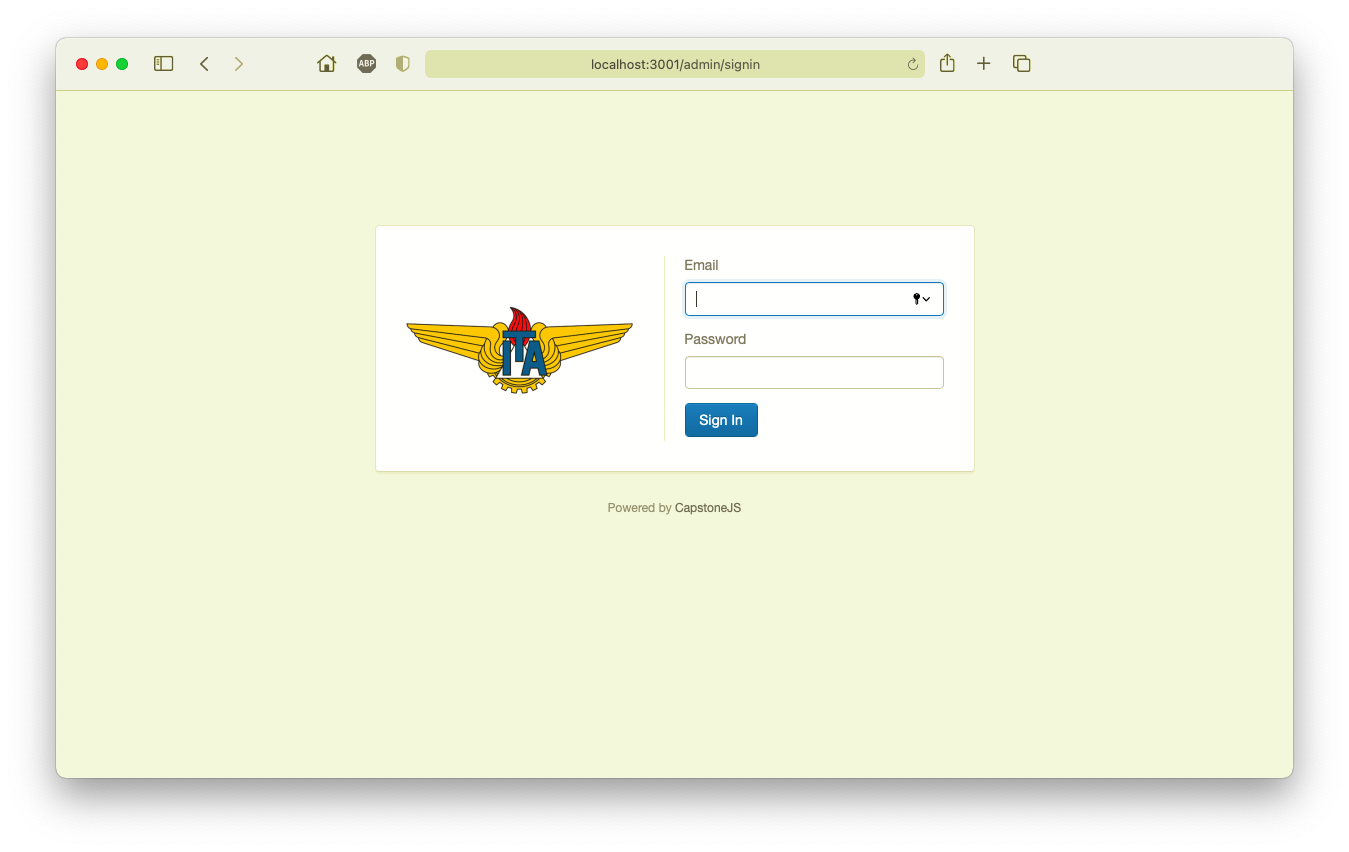
\includegraphics[width=.8\textwidth]{login}
    \caption{Tela de acesso ao Painel Administrativo}\label{RS0005:fig:login}
\end{figure}

\subsubsection{Integração de perfis via LDAP}

Em seguida, o usuário ``$admin$'' deve criar e manter os demais usuários que terão acesso ao Portal Administrativo. Em condições normais, nenhum usuário adicional deverá ter permissão para criar ou modificar os dados dos demais usuários (veja \cref{RS0005:fig:cadastro}).

A criação de perfis se dará também em duas etapas. Primeiramente é necessário definir os perfis desejados, e em seguida criar o grupo para cada perfil no servidor \gls{LDAP}. A definição de perfis se dá pela definição de regras de acesso no arquivo ``$rules.js$'' na pasta ``$config$'' contendo regras de acesso, o que veremos a seguir.

\begin{code}
    \inputminted[xleftmargin=20pt,fontsize=\footnotesize,breaklines,breakanywhere,linenos=true,label=editors.ldif]{YAML}{../RS0005/anexos/editors.ldif}
    \caption{Exemplo de definição de perfis para o LDAP}\label{RS0005:code:editores-ldif}
\end{code}

Na \cref{RS0005:code:editores-ldif} informamos ao serviço \gls{LDAP} os perfis que serão reconhecidos pelo controle de acesso. Observe também que os usuários para cada perfil já foram também informados (por exemplo, linhas $3$, $9$ até $11$ e $17$ até $18$).

\subsubsection{Integração de perfis via DB}

Na \cref{RS0005:fig:cadastro-usuario} podemos ver o atributo ``\textit{Role}'', onde são listados os papéis encontrados na configuração de \textbf{Regras de Acesso} (que veremos logo a seguir). Caso não haja um servidor \textbf{LDAP} disponível (ver (ver Guias do Desenvolvedor e do Operador), então este será o papel utilizado pelo para definir as regras de acesso do usuário.

Este atributo apresenta uma lista e o papel desejado pode ser escolhido. Diferentemente da definição de papéis via serviço \textbf{LDAP}, apenas um papel por usuário pode ser atribuído por intermédio do banco de dados.

\subsection{Regras de Acesso}

\begin{figure}[!ht]
    \centering
    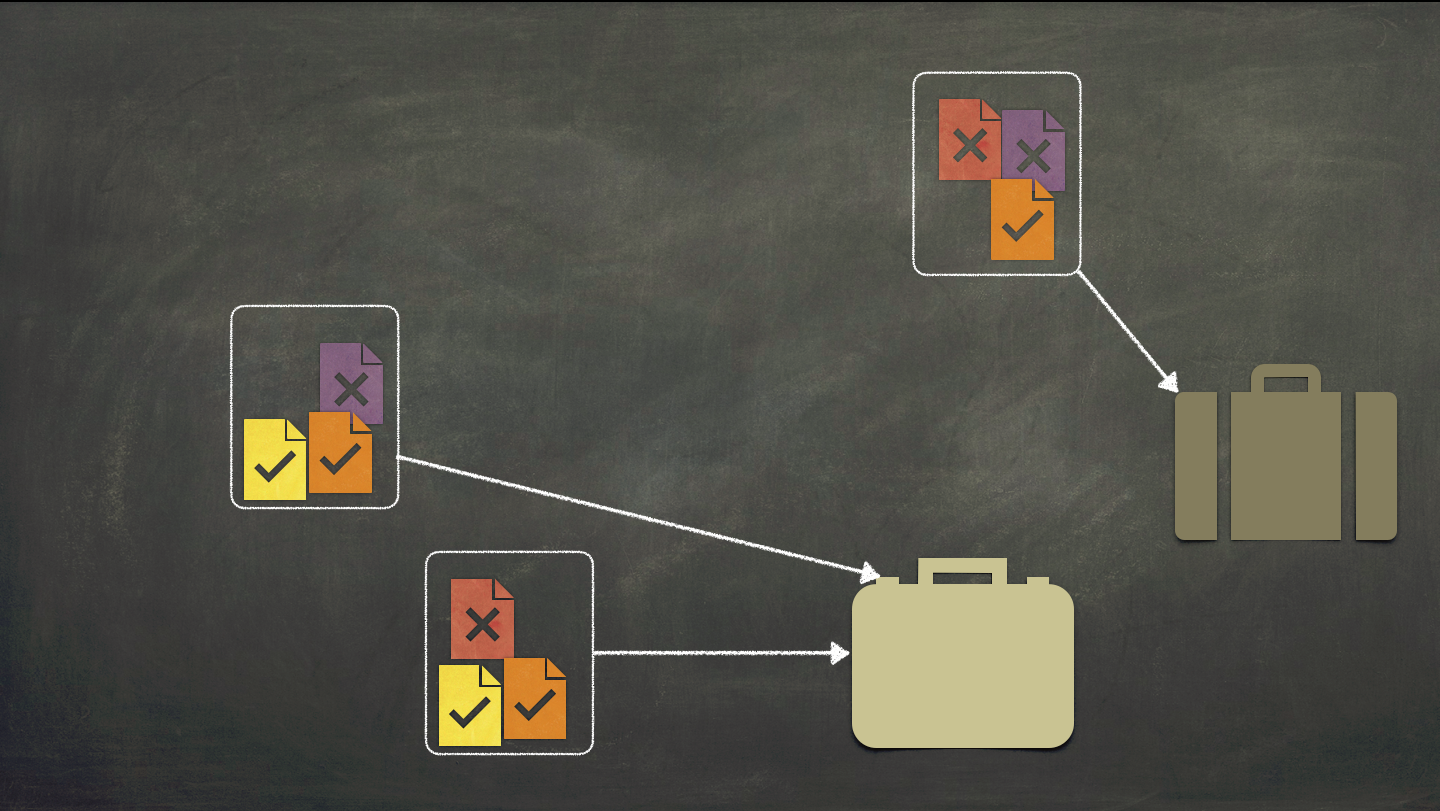
\includegraphics[width=.8\textwidth]{regras}
\end{figure}

Como dissemos anteriormente, a definição de perfis se dá pela definição de regras de acesso no arquivo ``$rules.js$'' na pasta ``$config$'' contendo regras de acesso.

Na \cref{RS0005:code:editores-ldif} podemos ver a definição do perfil ``$editor$'' que será atribuído ao usuário ``$maria$'' - a nossa editora geral e atribuida ao perfil na linha $3$. Esta definição reside no servidor \gls{LDAP}, onde temos as atribuições de usuários e os perfis correspondentes.

Porém, a definição de como o perfil deve ser atendido na aplicação é definida por meio de regras de acesso no arquivo ``$rules.js$'' na pasta ``$config$''. Na \cref{RS0005:code:regras-editor} mostramos uma definição de regras para o perfil ``$editor$''.

\begin{code}
    \inputminted[xleftmargin=20pt,fontsize=\footnotesize,breaklines,breakanywhere,linenos=true,label=rules.json,firstline=79,lastline=138]{JavaScript}{../RS0005/anexos/rules.js}
    \caption{Exemplo de regras de controle de acesso}\label{RS0005:code:regras-editor}
\end{code}

Na linha $79$ temos a definição do perfil, seguindo a estrutura de identificadores do serviço \gls{LDAP}. Em seguida temos o nome do recurso (exemplo na linha $80$ até $83$, ``$archives$'') e em seguida as permissões do perfil. As permissões possíveis são:

\begin{itemize}
    \item ``\textbf{$update:any$}'' - Atualização;
    \item ``\textbf{$delete:any$}'' - Exclusão;
\end{itemize}

Além destas permissões, o controle de acesso poderia controlar permissões para ``\textit{Leitura}'' (``\textbf{$read:any$}'') e ``\textit{Inclusão}'' (``\textbf{$create:any$}''), porém este tipo de acesso não é considerado pelo Painel Administrativo.

Além disto, o termo ``\textbf{$any$}'' chama a atenção. Existe ainda a possibilidade de definir se o acesso é de um recurso de todos usuários (``\textit{any}'') ou próprio (``\textit{own}''), porém, mais uma vez, o Painel Administrativo não considera a propriedade do recurso.

Finalmente, também podemos observar o valor ``\textbf{$[ '*' ]$}'' informado para o acesso. Seria possível informar uma lista de atributos do recurso para o qual o usuário teria acesso, e novamente, o Painel Administrativo não considera a segregação de atributos do recurso.

Em seguida, das linhas $84$ até $89$ temos definições de recursos com o nome em duas partes. Na primeira parte temos o nome do recurso (em nosso caso ``$archives$'') e na segunda parte um relacionamento deste recurso com outro recurso do Portal Administrativo. Temos por exemplo ``$archives.createdBy$'' e o acesso ``\textbf{$reference:any$}''. Antes de mais nada, veja na \cref{RS0005:code:archives} a definição de ``$archives$''.

\begin{code}
    \inputminted[xleftmargin=20pt,fontsize=\footnotesize,breaklines,breakanywhere,linenos=true,label=Archive.js]{JavaScript}{../RS0005/anexos/Archive.js}
    \caption{Modelo do recurso ``$Archives$''}\label{RS0005:code:archives}
\end{code}

Na linha $9$ temos a definição ``$track: true$'', que indica ao Painel Administrativo que desejamos ter registrados o nome do usuário que criou o registro (``$createdBy$''), do último usuário que o atualizou (``$updatedBy$'') e quando isto ocorreu (``$createdAt$'' e ``$updateAt$'' respectivamente). Estes atributos são diretamente ligados ao cadastro de usuários do Portal Administrativo.

Já um exemplo de ligação entre um documento e outro pode ser observado neste mesmo modelo de ``$archives$'' na linha $19$, onde existe a definição de uma relação entre estes ``\textit{archives}'' e o documento de ``\textit{Categories}'' (veja na linha $21$ na \cref{RS0005:code:category} a mesma definição, porém dentro do documento referenciado).

Este tipo de ligação existe portanto entre ``\textit{Archives}'' e os usuários do Portal Administrativo, e assim sendo é necessária a permissão para que quem for atualizar ``\textit{Archives}'' possa também atualizar esta relação.

\subsection{Segregação de Acesso}

Um dos principais objetivos de se ter um controle de acessos, é definir quem pode publicar no Portal Administrativo, e onde poderá publicá-las.

Para isto utilizaremos o recurso de definir regras de acesso e restrições no relacionamento do acesso.

No exemplo dado na \cref{RS0005:code:regras-editor}, o acesso ``\textbf{$reference:any$}'' recebe os valores ``\textbf{${ key: 'createdBy', value: '*' }$}'', que basicamente indica que o usuário pode referenciar qualquer valor que for atribuido em ``\textbf{createdBy}'' no documento ``$archives$''.

Porém para restringir a publicação no Portal Institucional, utilizaremos outro recurso que é informar um valor exato no par de atributos ``\textbf{$key$}'' e ``\textbf{$value$}''.

Isto irá funcionar pois daremos apenas aos usuário com perfil ``\textit{editor}'' a permissão de atualizar ``\textit{Menus}'', e em seguida definiremos exatamente o que cada menu irá apresentar por meio do atributo ``\textit{Categories}'', que define um grupo para classificar as informações publicadas no Portal Institucional.

Finalmente, será definido um perfil de usuário com permissão de criação de relações entre as publicações e determinadas categorias, como na \cref{RS0005:code:regras-posts-categories} que define uma regra que permite apenas publicar na categoria denominada ``$graduacao$'', em contraste com a \cref{RS0005:code:regras-ca}, que permite publicar com qualquer categoria.

\begin{code}
    \inputminted[xleftmargin=20pt,fontsize=\footnotesize,breaklines,breakanywhere,linenos=true,label=rules.json,firstline=155,lastline=157]{JavaScript}{../RS0005/anexos/rules.js}
    \caption{Exemplo de regras de controle de acesso}\label{RS0005:code:regras-posts-categories}
\end{code}

\begin{code}
    \inputminted[xleftmargin=20pt,fontsize=\footnotesize,breaklines,breakanywhere,linenos=true,label=rules.json,firstline=123,lastline=125]{JavaScript}{../RS0005/anexos/rules.js}
    \caption{Exemplo de regras de controle de acesso}\label{RS0005:code:regras-ca}
\end{code}

Além disto, o atributo ``$category$'' é obrigatório para as publicações (ver linha $36$ da \cref{RS0005:code:post} onde informamos ``$required: true, initial: true$'', que indica que o atributo é obrigatório e deve ser informado antes de ser possível criar um novo registro).

\begin{code}
    \inputminted[xleftmargin=20pt,fontsize=\footnotesize,breaklines,breakanywhere,linenos=true,label=Post.js]{JavaScript}{../RS0005/anexos/Post.js}
    \caption{Modelo de Publicação}\label{RS0005:code:post}
\end{code}

\subsubsection{Herdando regras}

É possível facilitar a criação de novos grupos de regras agrupando as regras comuns num único grupo e utilizando a cláusula ``$"\$extend": [ '<grupo-base>' ]$'', como no exemplo da \cref{RS0005:code:regras-extend}.

\begin{code}
    \inputminted[xleftmargin=20pt,fontsize=\footnotesize,breaklines,breakanywhere,linenos=true,label=extend.json]{JavaScript}{../RS0005/anexos/rules-extend.js}
    \caption{Exemplo de regras de controle de acesso comuns}\label{RS0005:code:regras-extend}
\end{code}

Na linha $39$ podemos ver que $editor-ipr$ ``extende'' as regras de ``$editor-base$''.

\subsection{Regras de Validação}

Uma extenção ao Controle de Acesso são as regras de validação.

Isto permite implementar papéis que possuem permissões específicas para determinados valores em atributos dos dados.

Para implementar um perfil que por exemplo possui permissão para inserir publicações com determinados valores, e outro perfil com permissões complementares, podemos fazer o seguinte:

\begin{code}
    \inputminted[xleftmargin=20pt,fontsize=\footnotesize,breaklines,breakanywhere,linenos=true,label=Rules.js]{JavaScript}{../RS0005/anexos/rules-validator.js}
    \caption{Perfis com regras de validação}\label{RS0005:code:rules-validator}
\end{code}

Entre as linhas $7$ e $12$ definimos um papel \textbf{editor-graduacao} e entre as linhas $13$ e $15$ o extendemos com exatamente as mesmas atribuições para o papel \textbf{revisor-graduacao}.

Na listagem abaixo complementamos os dois papéis definidos acima com regras de validação específicas para cada um dos papéis:

\begin{code}
    \inputminted[xleftmargin=20pt,fontsize=\footnotesize,breaklines,breakanywhere,linenos=true,label=Rules.js]{JavaScript}{../RS0005/anexos/validator.js}
    \caption{Perfis com regras de validação}\label{RS0005:code:validator}
\end{code}

Na linha $13$, o \textbf{editor-graduacao} implementa uma regra que diz:

\begin{displayquote}
    Permitir (\textit{ALLOW}) Publicações (\textit{posts}) que possuem os textos (\textit{isIn}) ``\textit{draft}'' e ``\textit{archived}'' no atributo ``\textit{state}''
\end{displayquote}

Já a linha $14$ o perfil implementa a regra:

\begin{displayquote}
    Negar (\textit{DENY}) Publicações (\textit{posts}) que possuem o texto (\textit{isIn}) ``\textit{published}'' no atributo ``\textit{state}''
\end{displayquote}

Em linhas gerais estamos \textbf{permitindo} ao perfil \textbf{editor-graduacao} possa gravar \textbf{publicações} com \textbf{estado} \textbf{rascunho} ou \textbf{arquivado} e \textbf{negando} no estado \textbf{publicado}.

Já o perfil \textbf{revisor-graduacao} implementa a regra:

\begin{displayquote}
    Permitir (\textit{ALLOW}) Publicações (\textit{posts}) que possuem os textos (\textit{isIn}) ``\textit{draft}'', ``\textit{published}'' e ``\textit{archived}'' no atributo ``\textit{state}''
\end{displayquote}

Neste caso estamos \textbf{permitindo} ao perfil \textbf{revisor-graduacao} gravar \textbf{publicações} em \textbf{qualquer} um dos \textbf{estado} possíveis.